%% Copernicus Publications Manuscript Preparation Template for LaTeX Submissions
%% ---------------------------------
%% This template should be used for copernicus.cls
%% The class file and some style files are bundled in the Copernicus Latex Package, which can be downloaded from the different journal webpages.
%% For further assistance please contact Copernicus Publications at: production@copernicus.org
%% https://publications.copernicus.org/for_authors/manuscript_preparation.html


%% Please use the following documentclass and journal abbreviations for preprints and final revised papers.

%% 2-column papers and preprints
\documentclass[esurf, manuscript]{copernicus}



%% Journal abbreviations (please use the same for preprints and final revised papers)

% Earth Surface Dynamics (esurf)
\usepackage{parskip}
\usepackage{subcaption}


%% \usepackage commands included in the copernicus.cls:
%\usepackage[german, english]{babel}
%\usepackage{tabularx}
%\usepackage{cancel}
%\usepackage{multirow}
%\usepackage{supertabular}
%\usepackage{algorithmic}
%\usepackage{algorithm}
%\usepackage{amsthm}
%\usepackage{float}
%\usepackage{subfig}
%\usepackage{rotating}
%\usepackage{amsmath}
\usepackage{float}     
\usepackage{placeins}  



\begin{document}

\title{TopoCurve: A python toolbox for discrete differential geometry on gridded surfaces}


% \Author[affil]{given_name}{surname}

\Author[1]{Taylor}{Schermer}%% correspondence author
\Author[1]{Joel}{Nash}
\Author[1]{Nathaniel}{Klema}
\Author[2]{Leif}{Karlstrom}

\affil[1]{Fort Lewis College}
\affil[2]{University of Oregon}

%% The [] brackets identify the author with the corresponding affiliation. 1, 2, 3, etc. should be inserted.

%% If an author is deceased, please mark the respective author name(s) with a dagger, e.g. "\Author[2,$\dag$]{Anton}{Smith}", and add a further "\affil[$\dag$]{deceased, 1 July 2019}".

%% If authors contributed equally, please mark the respective author names with an asterisk, e.g. "\Author[2,*]{Anton}{Smith}" and "\Author[3,*]{Bradley}{Miller}" and add a further affiliation: "\affil[*]{These authors contributed equally to this work.}".


\runningtitle{TopoCurve: A python toolbox for discrete differential geometry on gridded surfaces}

\runningauthor{Schermer et al.}

\received{}
\pubdiscuss{} %% only important for two-stage journals
\revised{}
\accepted{}
\published{}


\firstpage{1}

\maketitle

\begin{abstract}

\end{abstract}

\section{Summary}  
The calculation of topographic geometry metrics from Digital Elevation Models (DEMs) is fundamental to many Earth and planetary process studies. In particular, slope and curvature of topographic surfaces are linked to mass transport rates through analytical models, and thus are primary variables in studies that link topographic form to erosion rate variation. Making such studies directly comparable across the range of Earth and planetary settings requires the development data processing tools and workflows that minimize systematic error, and self-consistently calculate such metrics on surfaces of any orientation. `TopoCurve' is a Python package designed to analyze DEMs through a discrete differential geometry approach that minimizes projection error through calculation of the full curvature tensor at each pixel in a DEM. Through the calculation of invariant Mean and Gaussian curvatures this approach can be used to classify pixels into 9-distinct shape classes, providing a detailed picture of topographic geometry with potential applications in geomorphology, geomatics, geography, and adjacent Earth science fields.

\section{Statement of Need}
As both the resolution and availability of digital elevation datasets increases, so does their utility in identifying surface process signatures and their variation in both time and space \citep{roering2013you-440}.  While the connection between slope, curvature, and process models are well motivated by theory \citep{fernandes1997hillslope-8d8} common DEM processing workflows introduce systematic slope and curvature-dependent error that results from projecting topography onto a 2-D map plane \citep{minr2020comprehensive-9c9,klema2025discrete-964}, impacting the accuracy and utility of these connections. The workflow implemented in `TopoCurve` avoids some of this error through a formal surface-theory approach based on foundational ideas of Carl Frederick Gauss \citep{Gauss1902General1825}, which itself laid the groundwork for modern differential geometry and manifold theory \citep{pesic2007beyond}. The approach taken here follows that of \citet{klema2025discrete-964}, which provides a detailed implementation example. 

\section{State of the Field}
Several open‐source Python libraries implement differential‐geometry and surface analysis tools, but most are designed for triangle meshes or point clouds rather than gridded elevation models. Packages such as `LaPy' provide FEM‐based Laplace--Beltrami operators and curvature flows for mesh surfaces \citep{lapy2023LaPy}, while geometry‐processing libraries including `trimesh' and `PyMesh' offer curvature estimators, normals, and distance operators for 3D meshes \citep{trimesh2019, pymeshlibrary}. Point‐cloud toolkits such as `Open3D' and `PyTorch3D' supply additional intrinsic operators and geodesic utilities \citep{open3d2018, pytorch3d2020}. Although these libraries demonstrate broad interest in differential geometry within Python ecosystems, they are primarily designed for meshes rather than raster data.  

For geospatial applications, packages like `richdem', `whitebox', and `PyDEM' compute slope, aspect, and finite‐difference curvature on DEMs, but these approaches typically rely on planar finite-difference approximations that can introduce orientation and projection errors at high relief or resolution\citep{barnes2016richdem, jenness2013whitbox, balut2020pydem}. 

`TopoCurve'addresses this gap by adapting discrete differential‐geometry methods to DEM rasters, enabling reproducible, orientation‐independent calculations of mean and Gaussian curvature and associated shape classifications on topographic surfaces.


\section{Methods}
`TopoCurve' provides a comprehensive set of tools for both filtering DEM datasets and calculating intrinsic curvature invariants of topographic surfaces. The complete workflow for filtering and computing curvature invariants on a raw DEM can be seen in Figure \ref{fig:Flowchart}. Our approach to filtering is adapted from standard Fourier-based signal processing \citep{perron2008spectral-334}.  This workflow is well-suited for applications in which it is a priority not to suppress amplitude components within the region of interest \citep{Mcnutt1983,klema2025discrete-964}. Amplitude spectra are filtered using a half-Gaussian filter in the spectral domain. The spectrum is then inverse-transformed, and the window gives the original extent of the DEM.  This functionality is encapsulated in the `Spectral Filtering' object class, which allows the user to input wavenumber cutoffs for the filter and thus filter topography to a desired wavelength to isolate landscape features at a desired scale.  The effects of low-pass filtering topography using this approach can be seen in Figure \ref{fig:specfilt}, in which a sample DEM taken from the region of Purgatory Ski Area north of Durango, CO, is filtered to $200$ meters with half-Gaussian filter that begins at 150 m.

Once topography has been filtered to a desired wavelength, the Mean and Gaussian curvatures are calculated using the `CurveCalc' function within the `TopoCurve' object class. Many modern differential geometry approaches compute these surface curvature invariants through definition of the `Shape Operator matrix' \citep{Oneill2006diffgeometry,mynatt2007using-ba6}.  However, the same results with significantly shorter computation times are found using principal curvatures derived from quadratic equations that record how curvature varies with orientation at a given point.  A full summary of our mathematical approach can be found in \citep{klema2025discrete-964}. The principal curvatures can then be used on their own or be combined to find the Mean and Gaussian curvatures, defined respectively as the average and product of the two principal curvatures \citep{bergbauer2003how-56b}.  Maps of the mean and Gaussian curvatures can be seen in Figure \ref{fig:shapeclasses}.A and Figure \ref{fig:shapeclasses}.B respectively.\\

The Mean and Gaussian curvatures can be used together to sort each DEM pixel into one of the shape classes shown in Figure \ref{fig:shapeclasses}.C, providing a geometric representation of surface geometry. The colored shapes come directly from raw curvature measurements while the generation of points with zero Gaussian curvature requires definition of a threshold below which curvatures are taken to be zero \citep{mynatt2007using-ba6}.  While our code has the functionality for such thresholding we plot raw curvature values in our included figures.  Defining perfect saddles similarly requires defining a difference threshold below which Mean curvatures are taken to be the same.   The map view distribution of chape classes for our example DEM can be seen in Figure \ref{fig:shapeclasses}.D.  In this example we have not assigned a curvature threshold and so there are no pixels with zero Gaussian curvature. 

\section{Example Cases}
The `TopoCurve' repository includes three Jupyter notebooks with example implementations of the code.  The notebook '$example\_sphere.ipynb$' calculates curvature invariants on a sphere of radius $R$, where the Mean curvature everywhere is $1/R$ and the Gaussian curvature is $1/R^2$.  This example serves to demonstrate the ability of our method to accurately define curvature across a range of slopes relative to a horizontal plane. `$example.ipynb$' shows a basic topographic analysis workflow, and demonstrates how the `TopoCurve' package can be used to recreate Figures \ref{fig:specfilt} and \ref{fig:shapeclasses} from this report.  The notebook '$Area\_Binning.py$ follows the workflow of \citet{klema2025discrete-964} and can be used to recreate their Figure 7.


\FloatBarrier
\section{Figures}
  \centering

\begin{figure}[H]    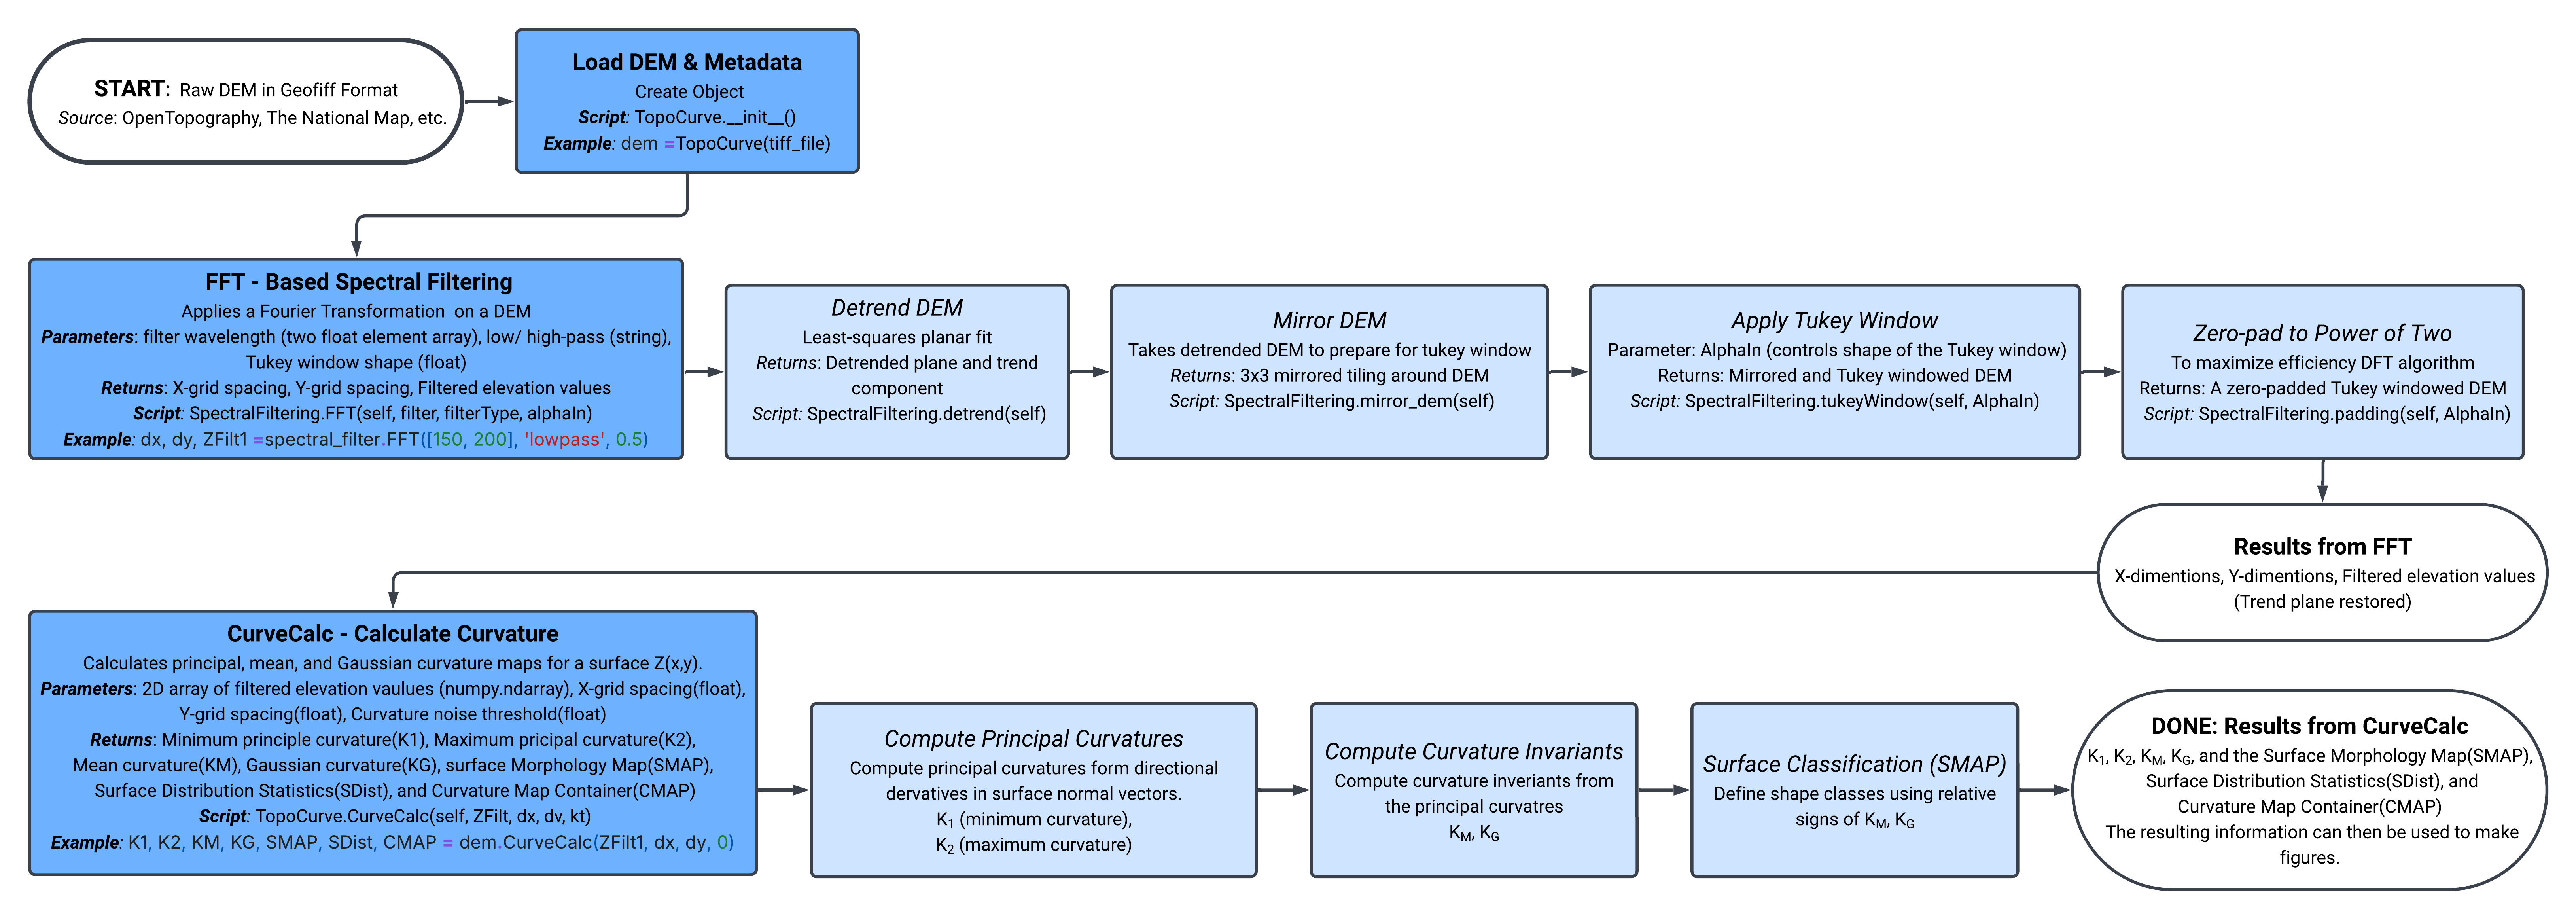
\includegraphics[width=0.9\textwidth]{Figures/Figure1.png}
    
    \caption{DEM processing workflow.}
    
    \label{fig:Flowchart}
\end{figure}

  
\begin{figure}[H]    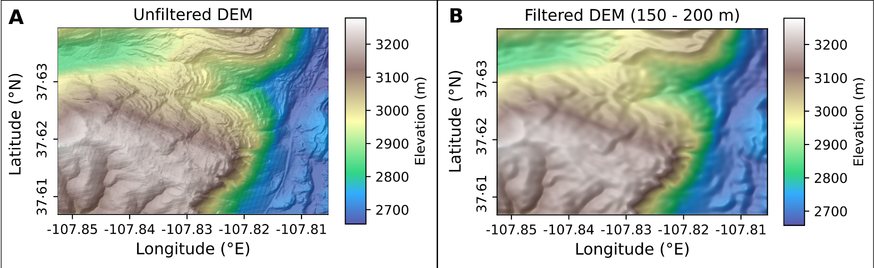
\includegraphics[width=0.9\textwidth]{Figures/Figure2.pdf}
    
    \caption{Example of the low-pass filtering pre-processing step applied to a 10 m resolution DEM taken of Purgatory ski area north of Durango, CO. \textbf{A.} The raw DEM. \textbf{B.} DEM filtered to 200 m wavelengths with a filter that tapers from wavelengths of 150 m, and which is applied to a mirrored DEM \citet{klema2025discrete-964}.}
    
    \label{fig:specfilt}
\end{figure}
\clearpage
\begin{figure}[H]
    \centering
    
\includegraphics[width=0.9\textwidth]{Figures/Figure3.pdf}
    \caption{ Curvature invariants and surface shape classes calculated on the filtered DEM from Figure \ref{fig:specfilt}. \textbf{A.} First principal curvature.  \textbf{B.} Second principal curvature. \textbf{C.} Shape classes derivable from Mean and Gaussian curvatures at each individual DEM pixel.  Figure from \citet{klema2025discrete-964}, however it is a modification of similar figures in \citet{bergbauer2003how-56b} and \citet{mynatt2007using-ba6}. \textbf{D.} Mean curvature. \textbf{E.} Gaussian curvature. \textbf{F.} Map of surface shape classes.}
    \label{fig:shapeclasses}
\end{figure}

\FloatBarrier



\bibliographystyle{copernicus}
\bibliography{references,references-2}

\end{document}
